\documentclass{article}
\usepackage[utf8]{inputenc}
\usepackage{graphicx}
\graphicspath{ {images/}}
\usepackage{wrapfig}
 
\title{TP1}
\author{RAJA GANAPATHY Srinivas ENGUIX Précillia}


\begin{document}
\maketitle
        
\section{Création de la fonction f (x)}


        Nous avons crée la fonction suivante:
$$f(x) = x^2 - x - 1$$

\begin{wrapfigure}{l}{1\textwidth}
        \centering
        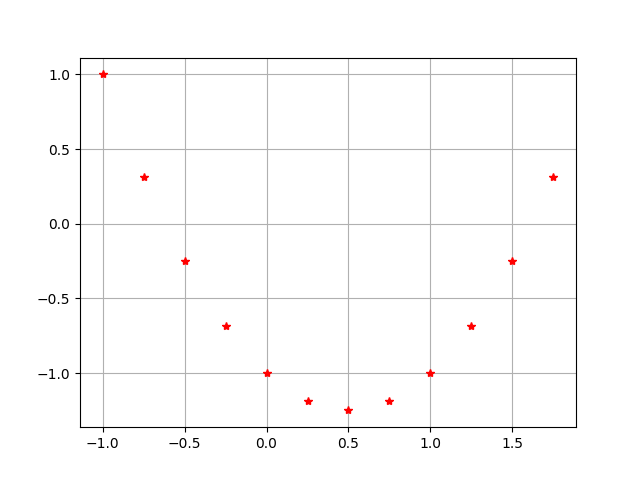
\includegraphics[width=0.75\textwidth]{fig1.png}
        $$ $$
\end{wrapfigure}

$$ $$
$$ $$
$$ $$
$$ $$
$$ $$
$$ $$
$$ $$
$$ $$
$$ $$
$$ $$
$$ $$
$$ $$

Pour pouvoir afficher le graphique de la fonction sur l'intervalle [-1,2], nous avons commencé par définir la ligne des abscisses à -1, le pas entre chaque point est de 0.25.
Pour construire le graphique nous avons utilisé une boucle while qui s'arrête quand x est inférieur à 2.
On affiche les points sur le graphique à l'aide de la commande print.
Pour afficher le graphique à l'écran, on utilise le module matplotlib.pylot.
On a observé la présence des deux zéros qui se situe à environ -0.61 et 1.61.
Ce sont les deux racines réels de la fonction f(x).

Pour pouvoir sauvegarder la figure nous utilisons la commande plt.savefig('nom du fichier.png'), mais nous constatons que lorsque nous changeons les paramètres du graphique, le changement n'a pas lieu directement, il met un certain temps à s'éxécuter.

\section{Utilisation de la méthode du point fixe}

Nous avons crée la fonction suivante:
$$g(x)= 1 + ( 1 / x )$$

\begin{wrapfigure}{l}{1\textwidth}
        \centering
        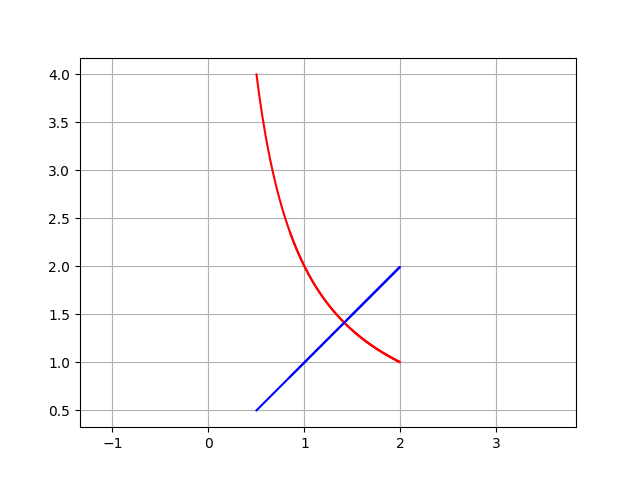
\includegraphics[width=0.75\textwidth]{fig2.png}
        $$ $$
\end{wrapfigure}

$$ $$
$$ $$
$$ $$
$$ $$
$$ $$
$$ $$
$$ $$
$$ $$
$$ $$
$$ $$
$$ $$
$$ $$


Nous observons que nous ne sommes plus obligé d'utiliser la boucle while pour créer la listes des points, la commande np.arange(x.debut,x.fin,pas) remplace l'intégralité de la boucle while.
Pour calculer les 25 premiers termes de la suite, nous avons utilisé la commande "i in range".
Pour la vérification nous sommes parti de f(x) :
$$f(x) = x^2 - x - 1 = 0 $$

$$<=> x^2 - x = 1$$

$$<=> x - 1 = (1 /= x)$$

$$<=> x = (1 / x) + 1 = g(x)$$

On remarque que les points converge vers 1.61 qui est l'un des deux zero de f.

Lors de l'affichage du graphe, on remarque que ça n'affiche que les graphiques de la fonction g, mais aussi celui de la fonction f.
$$ $$ 
\section{Implémentation de la fonction point fixe}
 
Lors de l'écriture de la fonction "point fixe", nous avons rencontré seulement des problémes de syntaxes et d'indentation, par exemple, nous oublions souvent les ":" à la fin des boucles et des def.
Lors de deux tests, nous avons remarqué dans le test 1 que les points partent de 2 et convergent vers 1.61 qui est un des 0 de f. Pour le test 2 les points partent de -0.6 et convergent vers 1.61. Donc les deux méthodes convergent.
$$ $$ 
\section{Méthode de Newton}

Nous n'arrivions pas à définir la fonction Newton car pour la commande "print('x vaut {0} et cpt vaut {1}').format(x,cpt)" entre la paranthése et le mot 'format' nous avions mit une virgule au lieu de mettre un point.
Cette fonction prend en compte un antécédent et la dérivée. Cette méthode peut vite devenir inutilisable pour certaines fonction dont la dérivée ne sera pas calculable.
Pour vérifier que les points fixes de g sont bien les zéros de f, nous avons fait les calculs à la main, et nous avons remarqué que ceux sont bien les zéros de f.
$$ $$ 
\section{Méthode de la sécante}

Dans la fonction sécante, on a rajouté un "x2" pour avoir plus de visibilité. On peut observer que pour la fonction sécante, nous avons besoin de 2 antécédents pour pouvoir calculer la valeur suivante. Pour la fonction newton nous n'avons besoin que d'un seul antécédent, mais nous devons utiliser la dérivée, pour calculer la valeur suivante.
Or, pour certaines fonction, il est impossible de calculer la dérivée, donc la fonction sécante est bien meilleure.
$$ $$ 
\section{Méthode de dichotomie}

La fonction dichotomie n'était pas la fonction la plus compliquée à créer, car on avait déjà étudié cette fonction en algorithme.
Nos tests ne fonctionnaient pas, nous ne savions pas si c'était la fonction elle-même qui ne fonctionnait pas ou si il y avait un probléme dans les tests directement, car ça compilait mais nous n'avions pas l'affichage des tests. Finalement nous avons compris que l'erreur venait des tests, nous n'avions pas défini a, b, et epsi. Une fois ces paramétres défini, les tests ont fonctionnés.
$$ $$ 
\section{Analyse de la séance de TP}

Durant ces deux séances de TP, nous avons d'abord appris à coder en python. Ce langage informatique est beaucoup plus simple que le langage C, car il demande beaucoup moins de structures. Les erreurs sont plus simple à corriger. Nous pouvons donc avancer plus rapidement sur le TP.
De plus, nous avons appris à rédiger un rapport en latex. On a fait des recherches sur internet pour mieux utiliser ce format (rajout d'accent, ajout de graphique, ajout de formule mathématique). Mais nous ne maitrisons pas completement ce format, au fil des TP il faudra faire d'avantage de recherches.






\end{document}
